\section*{Analiza wielkości wyjaśnień}

W tej sekcji przeprowadzono szczegółową analizę wpływu wielkości obiektu na rozmiar obszaru wyjaśniania wygenerowanego przez metody LIME, SHAP i GradCAM.
Badanie miało na celu zgłębienie, jak różne metody XAI reprezentują istotność różnych części obrazu w zależności od wielkości obiektów na zdjęciach.
Kluczowe było zrozumienie, jak metody XAI regują na obiekty o różnej wielkości.

\begin{figure}[h]
	\centering
	\begin{subfigure}[b]{0.45\textwidth}
		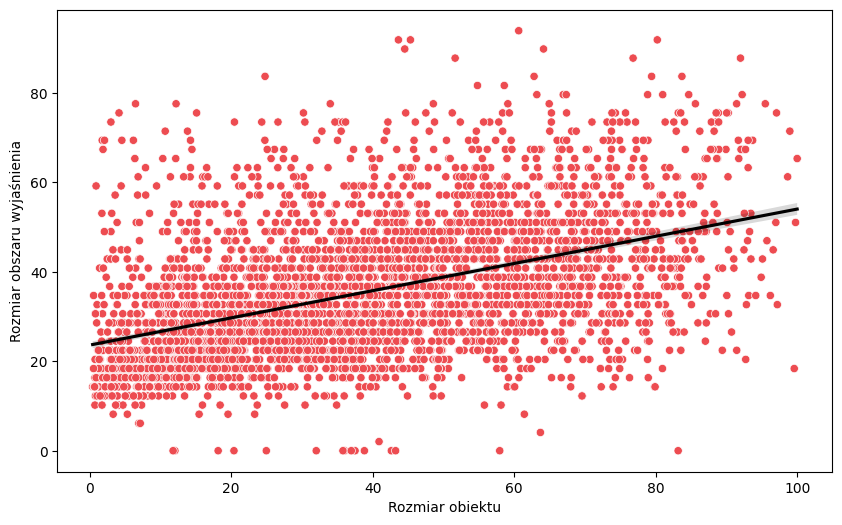
\includegraphics[width=.9\textwidth]{img/size_exp_gradcam}
	\end{subfigure}
	\begin{subfigure}[b]{0.45\textwidth}
		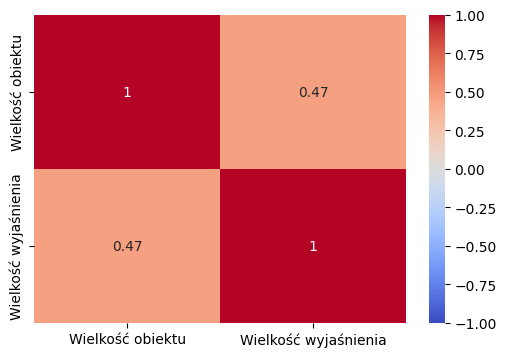
\includegraphics[width=.9\textwidth]{img/size_exp_gradcam_corr}
	\end{subfigure}
	\caption{Zależność między rozmiarem obiektu, a rozmiarem obszaru wyjaśnienia GradCAM}
	\label{rys:size_exp_gradcam}
\end{figure}
\begin{figure}[h]
	\centering
	\begin{subfigure}[b]{0.45\textwidth}
		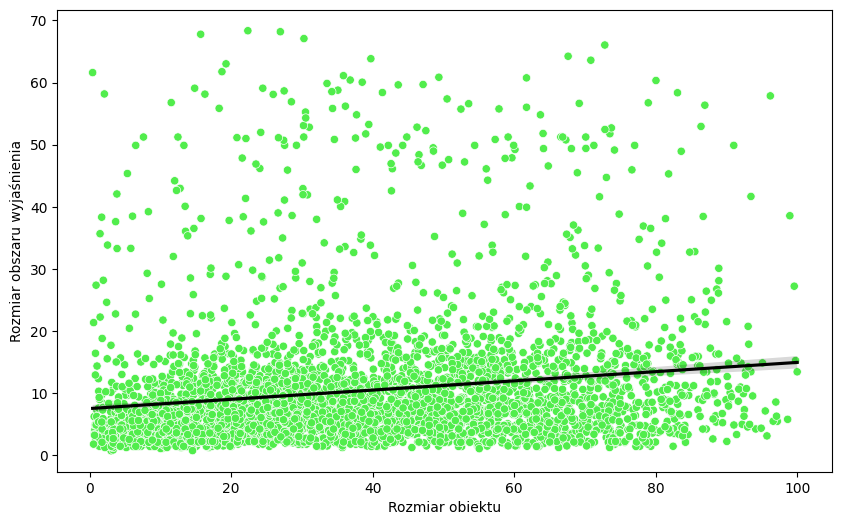
\includegraphics[width=.9\textwidth]{img/size_exp_lime}
	\end{subfigure}
	\begin{subfigure}[b]{0.45\textwidth}
		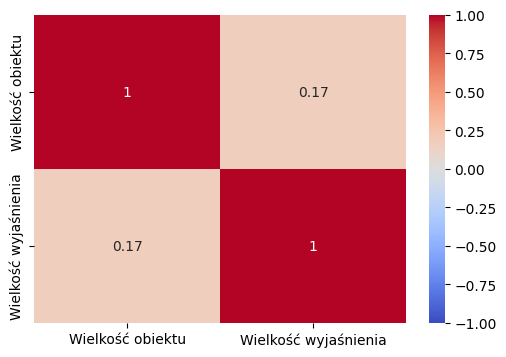
\includegraphics[width=.9\textwidth]{img/size_exp_lime_corr}
	\end{subfigure}
	\caption{Zależność między rozmiarem obiektu, a rozmiarem obszaru wyjaśnienia LIME}
\end{figure}
\begin{figure}[h]
	\centering
	\begin{subfigure}[b]{0.45\textwidth}
		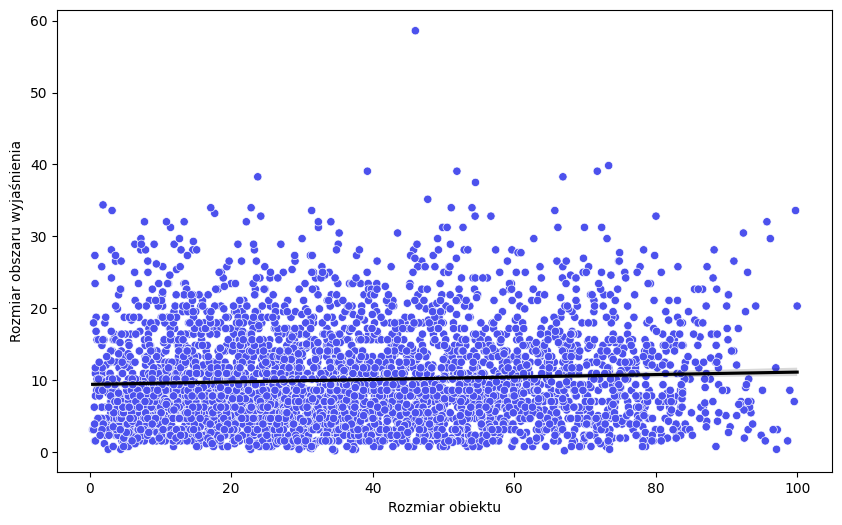
\includegraphics[width=.9\textwidth]{img/size_exp_shap}
	\end{subfigure}
	\begin{subfigure}[b]{0.45\textwidth}
		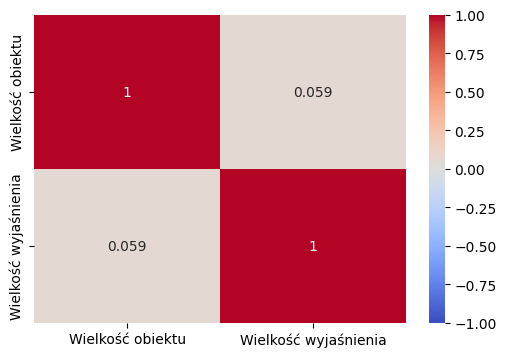
\includegraphics[width=.9\textwidth]{img/size_exp_shap_corr}
	\end{subfigure}
	\caption{Zależność między rozmiarem obiektu, a rozmiarem obszaru wyjaśnienia SHAP}
	\label{rys:size_exp_shap}
\end{figure}

Wyniki zostały przedstawione za pomocą wykresów (Rys. \ref{rys:size_exp_gradcam}-\ref{rys:size_exp_shap}), które wizualizują zależności między wielkością obiektów, a rozmiarem wyjaśnień generowanych przez poszczególne metody.
Na końcu pracy, w Dodatku \ref{app2}, znajdują się przykłady obrazów z zaznaczonymi wyjaśnieniami.
Dodatek ten zawiera przykłady, gdy wielkość wyjaśnienia jest zbliżona do rzeczywistej wielkości obiektu na obrazie, jak i przypadki, gdzie występuje znacząca różnica między tymi wartościami.
Takie podejście pozwala lepiej zrozumieć i interpretować otrzymane wyniki.

Analiza wpływu wielkości obiektu na rozmiar wyjaśnień generowanych przez metody XAI wykazał, że wyjaśnienia \textbf{GradCAM} charakteryzuje największą korelacje między wielkością obszaru obiektu a wielkością wyjaśnienia.
Dodatkowo na wykresie punktowym (Rys. \ref{rys:size_exp_gradcam}) widoczne jest, silne skorelowanie wyjaśnień GradCAM z rozmiarami warstwy konwolucyjnej, co oznacza ograniczenia tej metody.

\textbf{LIME} wykazał niższą korelację niż GradCAM, generując wyjaśnienia często o małych rozmiarach, zazwyczaj poniżej 25\% rozmiaru obrazu.
Wysoka czułość LIME na dobór parametrów może mieć istotny wpływ na ten wynikj.

Natomiast \textbf{SHAP} wykazał najniższą korelacje lub praktycznie jej brak.
Obszary wyjaśnień SHAP są również zazwyczaj małe, co jest zgodne z obserwacjami dla LIME.
Wybór odpowiednich parametrów mógł znacząco wpłynąć na wyniki.

\vspace{1cm}
Analiza wielkości wyjaśnień dla metod GradCAM, LIME i SHAP pokazuje, że każda z tych metod ma różne podejścia do generowania obszarów kluczowych na obrazach.
GradCAM charakteryzuje się największą spójnością wielkości wyjaśnień, odpowiadającej rzeczywistej wielkości obiektów, co może być istotne w zastosowaniach praktycznych.
LIME i SHAP natomiast mniejsze wyjaśnienia, co może być spowodowane doborem parametrów, w celach praktycznych parametry powinny być dobierane osobno dla każdego przypadku.

